\documentclass{article}
\usepackage{amsmath}
\usepackage{amssymb}
\usepackage{graphicx}
\usepackage{hyperref}
\usepackage[version=4]{mhchem}


\begin{document}
\section*{Problem}
In \(\triangle A B C, A B=5 . A C=9 . A D\) is the median on side \(B C\). How many integer values are there of \(A D\) ?\\
\centering
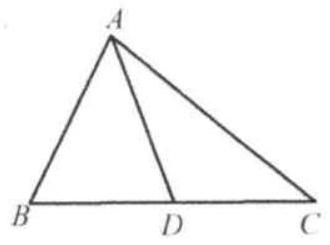
\includegraphics[width=\textwidth]{images/027(2).jpg}

\section*{Solution}
4.
Extend \(A D\) to \(E\) such that \(A D=D E\).\\
Connect \(B E\).\\
Since \(D E=A D, \angle B D E=\angle C D A . B D=D C\).\\
Thus \(\triangle B D E \cong \triangle C D A, B E=A C=9\).\\
By the triangle inequality theorem,\\
\(9-5<A E<9+5 \quad \Rightarrow \quad 4<2 A D<14 \Rightarrow 2<A D<\)\\
\centering
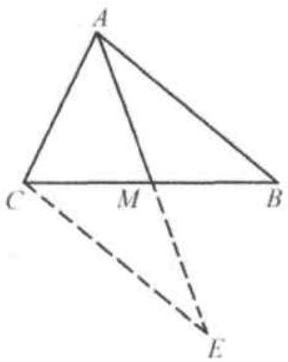
\includegraphics[width=\textwidth]{images/029(1).jpg}\\
\(E\)

7.

There are four possible values: \(3,4,5\), and 6 .

\end{document}
